
The model we consider is the current draft specification (cite here) of ECMAScript standard. 
This draft as far as the memory model goes has remained unchanged, so we believe our work will also be of use to those working on thismodel. 
The specification is claimed to be axiomatic by definition, which should, in our view remove the complexities of the rest of thestandard from the semantics of the model.
However, as we noted, there were quite some concerns with it: 

\paragraph{The Model is Quite Algorithmic}
    Although the standard states that the model is not supposed to be operational, the specifications of the model state otherwise. 
    There are quite a few abstract operations which are not necessary to understand the semantics of the model. 
    As an example, consider one of the Axioms of the model below as stated by the standard. 
    \begin{figure}[H]
        \centering 
        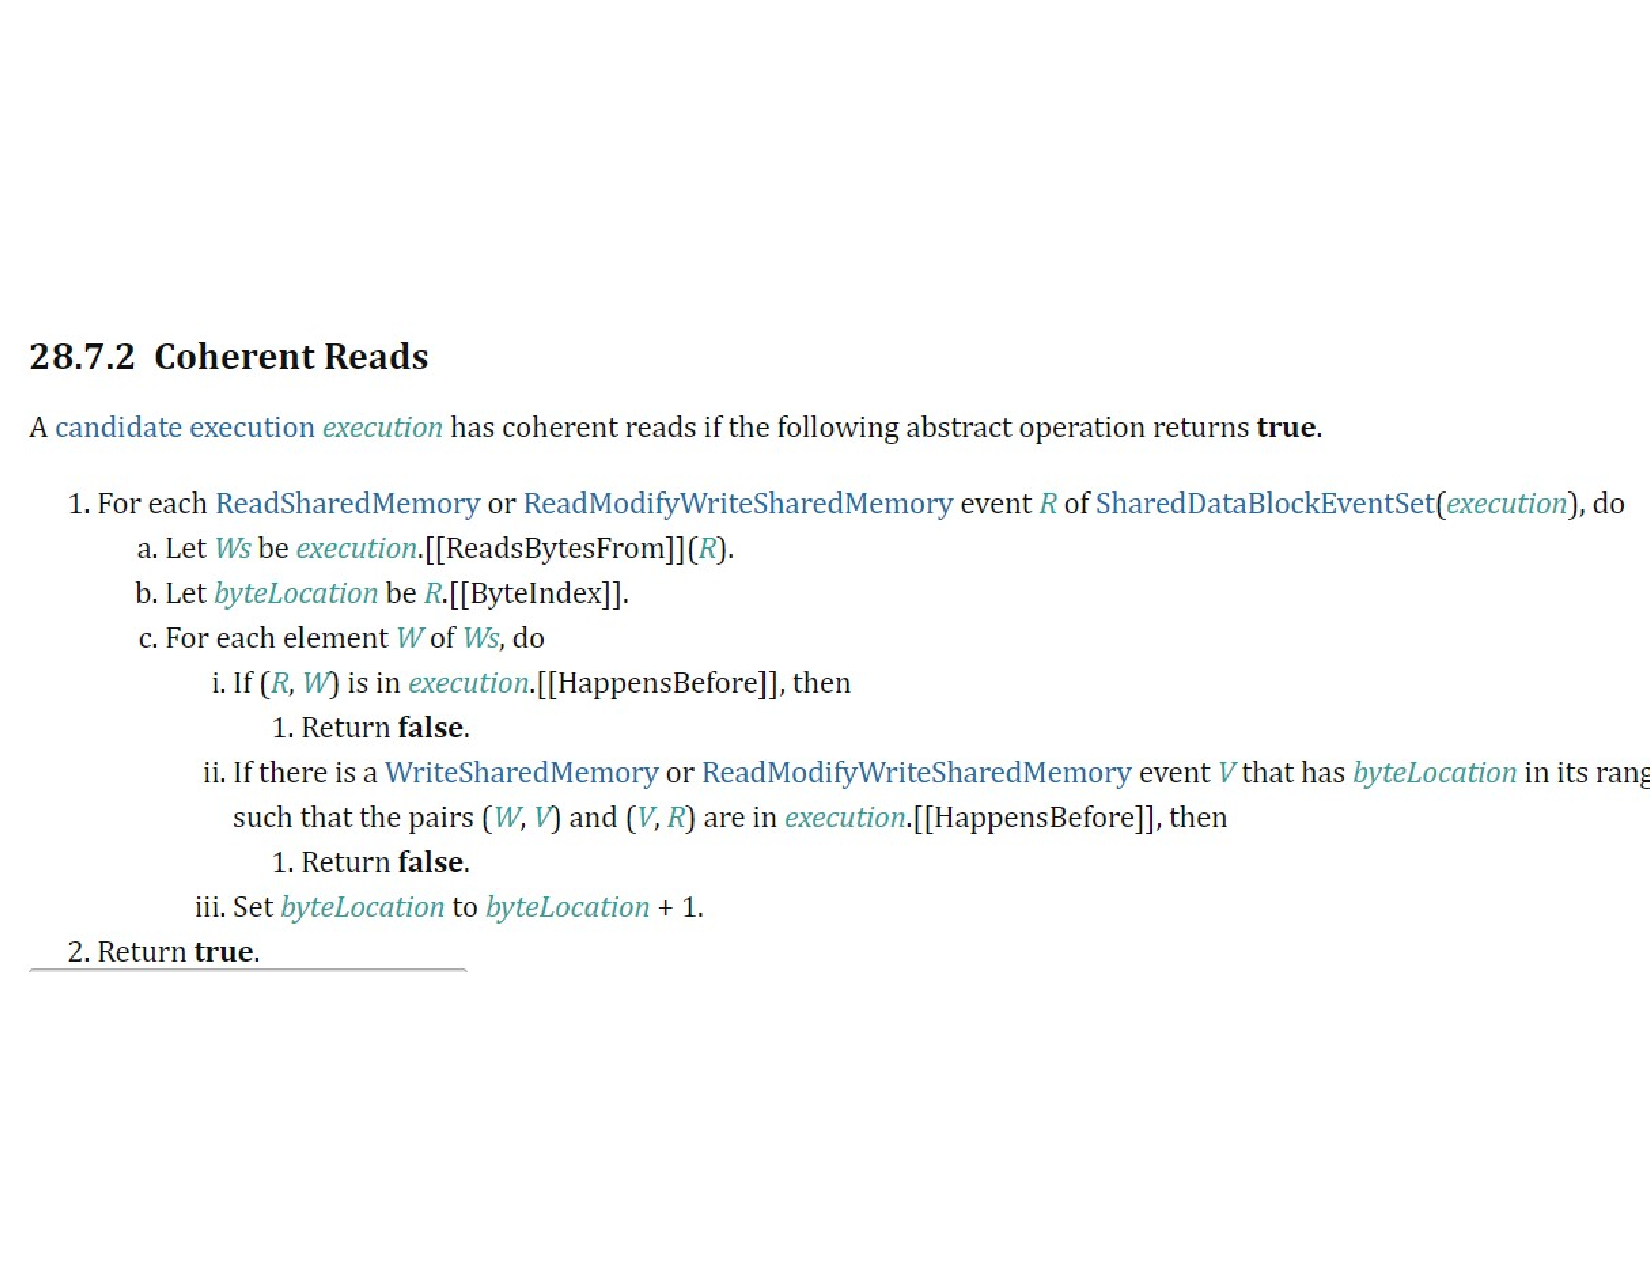
\includegraphics[scale=0.6]{4.ECMAScriptMemoryModel/ECMAScriptStdCoherentReads.pdf}
        \caption{The ECMAScript specification for Coherent Reads.}
    \end{figure}
    The above axiom is specified as a return value to an abstract operation. While understanding this requires one to know thedefintions of $Ws$, $execution$, $SharedDataBlockEventSet$ abstract operation, etc. we believe this is not needed as to understandwhat the axiom is about, which informally can be stated as below in two points:
    \begin{itemize}
        \item A read's value cannot come from a write that has happened after it. 
        \item A read's value cannot come from a write that has been overwritten by some other write.  
    \end{itemize}
    Axiomatically, we define the above two points using simple binary relations that we derive from the specification to exist amongevents. The entire specification is structured in a similar way. 

\paragraph{Certain Unnecessary Definitions}
    
    Certain abstract operations are not required to capture the semantics of the model. 
    One such example is in the figure below:
    \begin{figure}[H]
        \centering 
        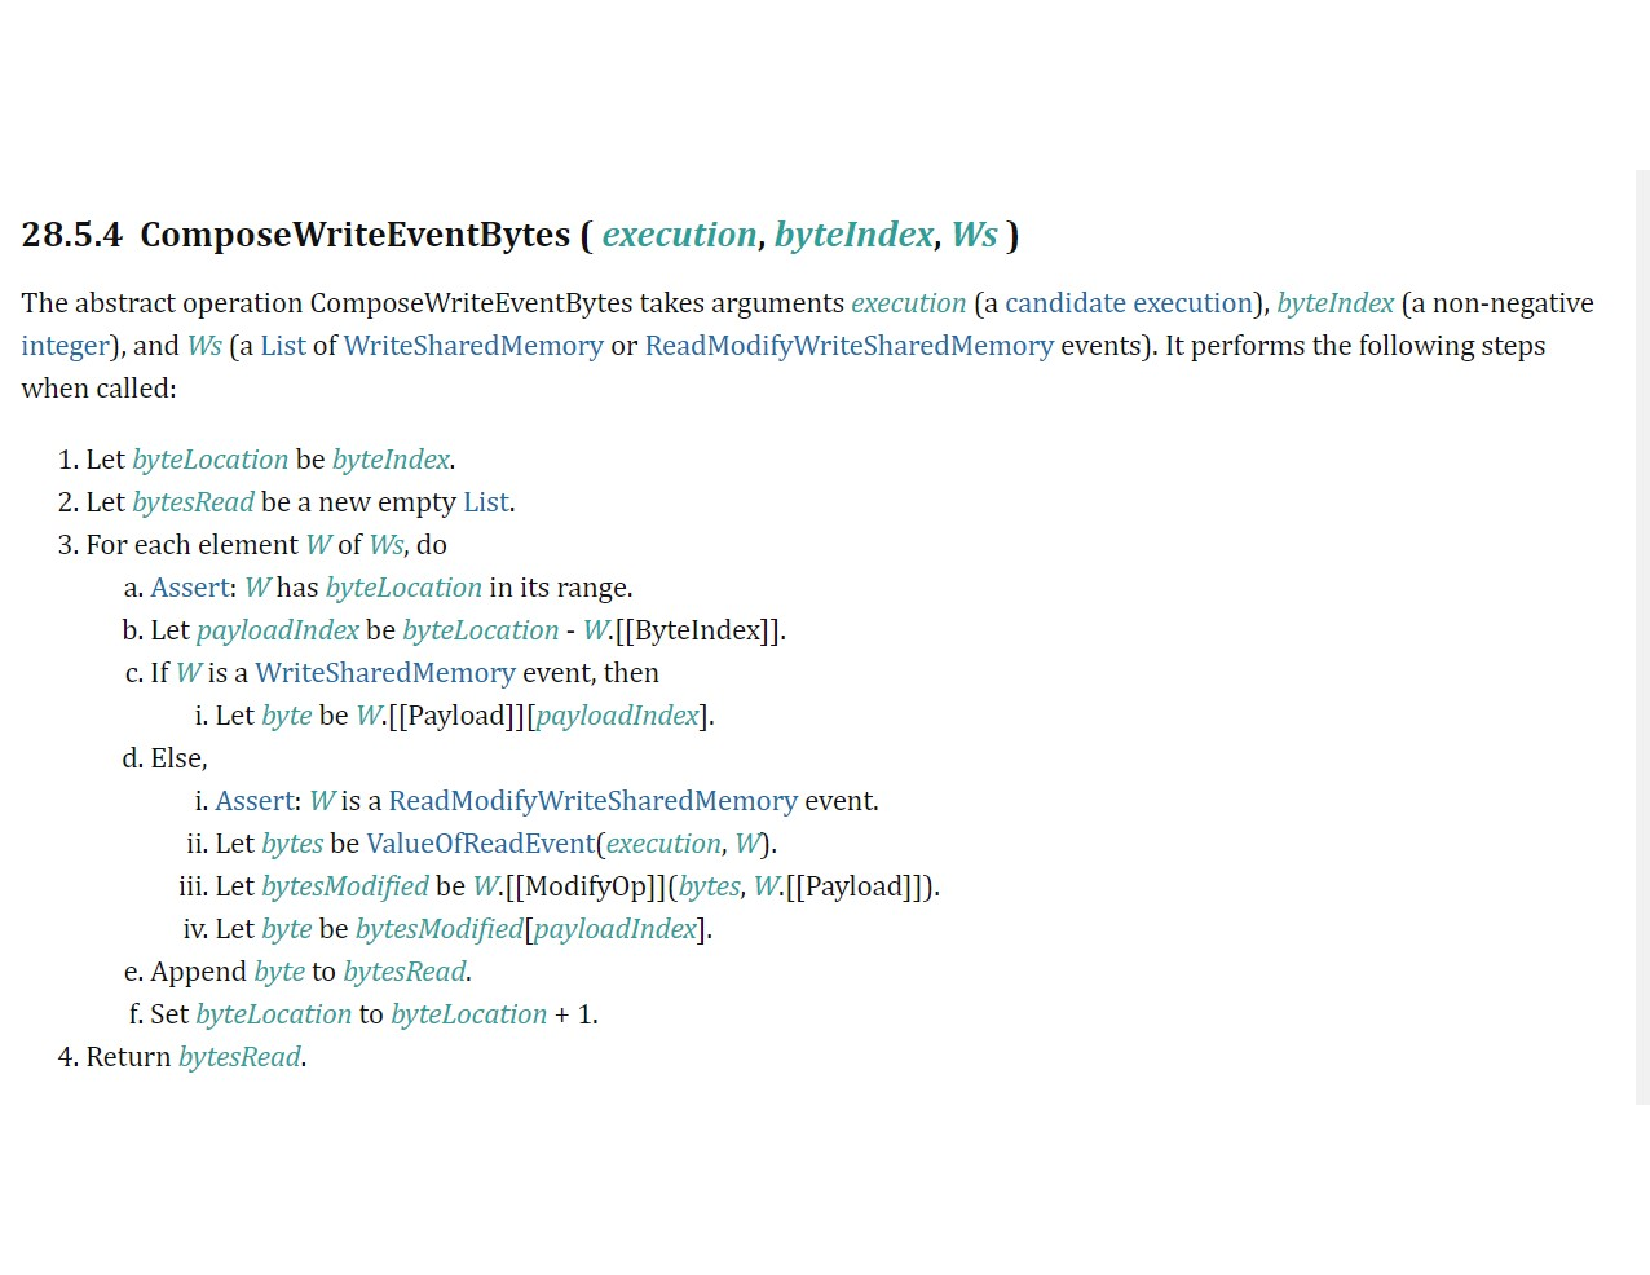
\includegraphics[scale=0.6]{4.ECMAScriptMemoryModel/ECMAScriptStd.pdf}
        \caption{The ECMAScript specification for Compose Write Event Bytes.}
    \end{figure}
    The above figure is the definition of an abstract operation. To understand what this operation does, one must know the meaning of the terms $ModifyOp$, $Payload$, the list $Ws$, and also know what the argument $ByteIndex$ signifies. 
    In its essence, the above operation gives the read-values read by a single write by collecting the values from their corresponding writes. 
    We realized that one need not know this operation nor understand its function as it does not play a role in the semantics of the model. 
    Other such abstract operations are $ValueOfReadEvent$ and $ValidChosenReads$. 

\paragraph{Still a bit verbose}
    
    The entire model, is still quite verbose, which makes it difficult to understand the main objective of the model semantics. 
    The following figure is the std specification of another Axiom 
    \begin{figure}[H]
        \centering 
        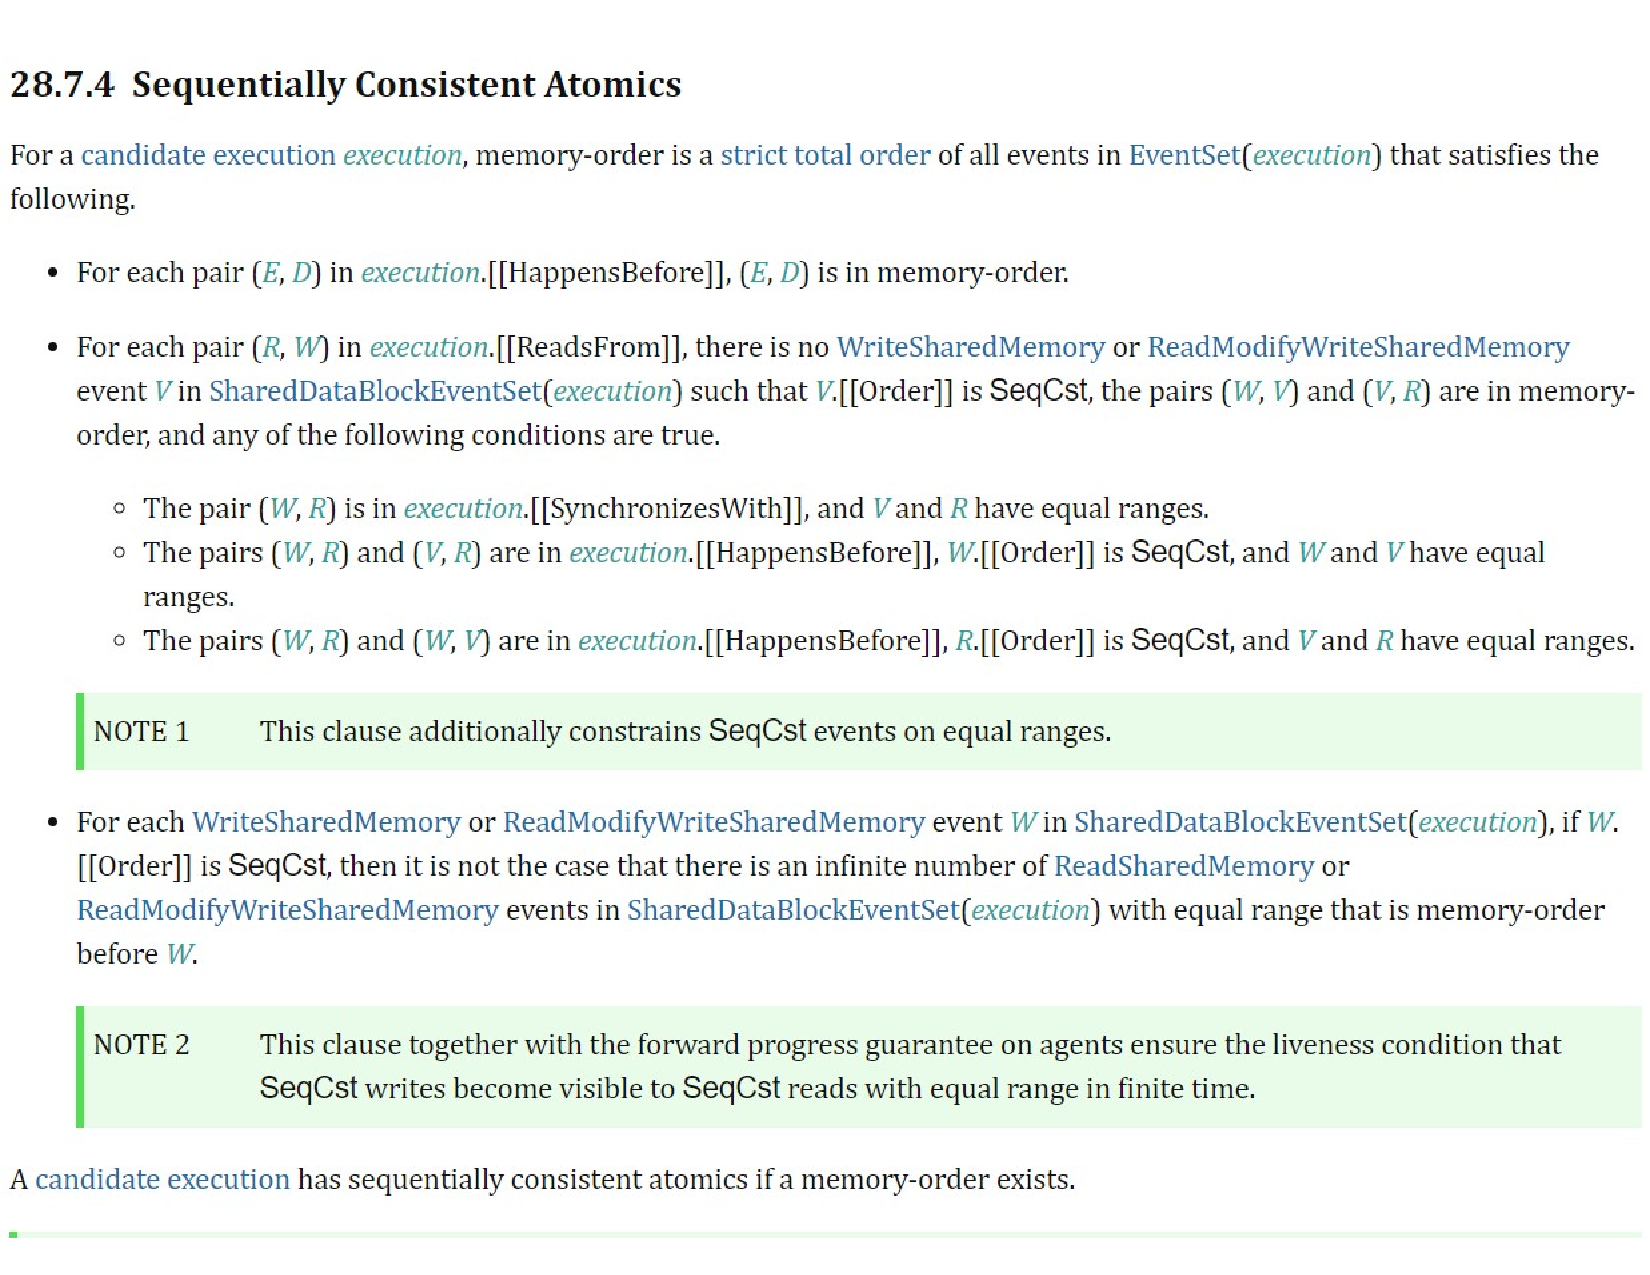
\includegraphics[scale=0.6]{4.ECMAScriptMemoryModel/ECMAScriptStdSeqCnsAt.pdf}
        \caption{The ECMAScript specification for Sequentially Consistent Atomics axiom.}
    \end{figure}
    The above figure, though written concisely, in our view still makes it difficult to understand. 
    We reduced the above entire axiom into three main patterns using binary relations that should not exist in any execution of a program. 
    While the latter part is less of a semantic specification and more of a programming guideline while using relaxed memory accesses.(one can make countless counter-examples for this.) 

Given the above concerns about the model specification in the standard, we formalized it axiomatically in the form of binary relations over events involved and axioms that place restrictions on some of them using the others. 

